\documentclass{ximera}

% These macros are automatically generated from the "macros"
% XML element.  Make permanent edits there.
%
% History
%   2004/01/01  Initiated for FCLA, evolved from there
%   2006/09/17  Converted  _, ^  to \sb, \sp for TeX4ht
%   2014/02/01  Updated for MathBook XML projects
%               Obsolete in FCLA: \codeindent, \computerfont, \define
%               Change: MathJax wants \lt, so replaced by \lteval
%   2014/02/22  New: \orderof, \reals, \per
%   2015/08/16  Incorporated into MathBook XML version of FCLA
%
%%%%%%%%%%%%%%%%%%%%%
%
%     Conveniences
%
%%%%%%%%%%%%%%%%%%%%%
%
%  Order of (asymptotically limit of fraction is 1)
%  Usage: \orderof{some function}
%
\newcommand{\orderof}[1]{\sim #1}
%
%  Integers
%  Usage:  \Z
\newcommand{\Z}{\mathbb{Z}}
%
%  Real numbers, as set of scalars
%  Usage:  \reals
\newcommand{\reals}{\mathbb{R}}
%
%  n-space over real field
%  Usage: \complex{integer-dimension}
\newcommand{\real}[1]{\mathbb{R}^{#1}}
%
%  Complex numbers, as set of scalars
%  Usage:  \complexes
\newcommand{\complexes}{\mathbb{C}}
%
%  n-space over complex field
%  Usage: \complex{integer-dimension}
\newcommand{\complex}[1]{\mathbb{C}^{#1}}
\newcommand{\CC}{\mathbb{C}}
%
%  Complex conjugation (scalar, vector, matrix)
%  Usage: \conjugate{object}
\newcommand{\conjugate}[1]{\overline{#1}}
%
%  Complex number modulus
%  Usage: \modulus{a+bi}
%  Presumes math mode
\newcommand{\modulus}[1]{\left\lvert#1\right\rvert}
%
%  Zero vector
%  Usage: \zerovector
\newcommand{\zerovector}{\vect{0}}
%
%  Zero matrix
%  Usage: \zeromatrix, use a subscript when size is important
\newcommand{\zeromatrix}{\mathcal{O}}
%
%  Inner product (brackets, not quadratic form)
%  Usage: \innerproduct{a-vector}{a-vector}
\newcommand{\innerproduct}[2]{\left\langle#1,\,#2\right\rangle}
%
%  Norm of a vector
%  Usage: \norm{a-vector}
\newcommand{\norm}[1]{\left\lVert#1\right\rVert}
%
%  Dimension
%  Usage: \dimension{vector-space-letter}
\newcommand{\dimension}[1]{\dim\left(#1\right)}
%
%  Nullity
%  Usage: \nullity{matrix-or-lintrans-letter}
\newcommand{\nullity}[1]{n\left(#1\right)}
%
%  Rank
%  Usage: \rank{matrix-or-lintrans-letter}
\newcommand{\rank}[1]{r\left(#1\right)}
%
%  Direct sum
%  Usage: \ds between a couple of subspaces
%
\newcommand{\ds}{\oplus}
%
%  Determinant of a matrix (functional)
%  Usage: \detname{A}
\newcommand{\detname}[1]{\det\left(#1\right)}
%
%  Determinant of a matrix (vertical bars)
%  Usage: \detbars{A}
\newcommand{\detbars}[1]{\left\lvert#1\right\rvert}
%
%  Trace of a Matrix
%  Usage: \trace{matrix name}
\newcommand{\trace}[1]{t\left(#1\right)}
%
%  Square Root of a Matrix
%  Usage: \sr{a-matrix}
\newcommand{\sr}[1]{#1^{1/2}}
%
%%%%%%%%%%%%%%%%%%%%%
%
%     Subspace Constructions
%
%%%%%%%%%%%%%%%%%%%%%
%
%  Span of a set of vectors
%  \span and \sp are used by TeX for other things
%  Usage: \spn{set-of-vectors}
\newcommand{\spn}[1]{\left\langle#1\right\rangle}
%
%  Null space of a matrix
%  Usage:  \nsp{A}
\newcommand{\nsp}[1]{\mathcal{N}\!\left(#1\right)}
%
%  Column space of a matrix
%  Usage:  \csp{A}
\newcommand{\csp}[1]{\mathcal{C}\!\left(#1\right)}
%
%  Row space of a matrix
%  Usage:  \rsp{A}
\newcommand{\rsp}[1]{\mathcal{R}\!\left(#1\right)}
%
%  Left null space of a matrix
%  Usage:  \lns{A}
\newcommand{\lns}[1]{\mathcal{L}\!\left(#1\right)}
%
%  Orthogonal complement of a vector space
%  Avoiding TeX's \perp
%  Usage:  \per{A}
\newcommand{\per}[1]{#1^\perp}
%
%%%%%%%%%%%%%%%%%%%%%
%
%     Systems of Equations
%
%%%%%%%%%%%%%%%%%%%%%
%
%  In-line form of an augmented matrix for a system of equations
%  Usage: \augmented{coefficient-matrix}{constant-vector}
\newcommand{\augmented}[2]{\left\lbrack\left.#1\,\right\rvert\,#2\right\rbrack}
%
%  Notation for a linear system before introducing matrix multiplication
%  Usage: \linearsystem{coefficient-matrix}{constant-vector}
\newcommand{\linearsystem}[2]{\mathcal{LS}\!\left(#1,\,#2\right)}
%
%  Notation for a homogenous system before introducing matrix multiplication
%  Usage: \homosystem{coefficient-matrix}
\newcommand{\homosystem}[1]{\linearsystem{#1}{\zerovector}}
%
%%%%%%%%%%%%%%%%%%%%%
%
%     Row Operations, Echelon Form
%
%%%%%%%%%%%%%%%%%%%%%
%
% Row operations on matrices
%
% Three commands to shorten up descriptions of gaussian elimination
%
% Usage: \rowopswap{row-i}{row-j}
% Usage: \rowopmult{scalar}{row-i}
% Usage: \rowopadd{scalar}{row-multiplied}{row-added-to}
\newcommand{\rowopswap}[2]{R_{#1}\leftrightarrow R_{#2}}
\newcommand{\rowopmult}[2]{#1R_{#2}}
\newcommand{\rowopadd}[3]{#1R_{#2}+R_{#3}}
%
% Mark leading 1's in echelon form with fbox
% Usage: \leading{a-1-usually}
\newcommand{\leading}[1]{\fbox{#1}}
%
%  Row-reduce arrow
%  Usage:  \rref inbetween a matrix and its reduced row-echelon form
\newcommand{\rref}{\xrightarrow{\text{RREF}}}
%
%  Elementary Matrices
%  Usage: \elemswap{subscript}{subscript}
%  Usage: \elemmult{scalar}{subscript}
%  Usage: \elemadd{scalar}{subscript-mult}{subscript-target}
%
\newcommand{\elemswap}[2]{E_{#1,#2}}
\newcommand{\elemmult}[2]{E_{#2}\left(#1\right)}
\newcommand{\elemadd}[3]{E_{#2,#3}\left(#1\right)}
%
%%%%%%%%%%%%%%%%%%%%%
%
%     2-D Constructions (Lists, Vectors, Matrices)
%
%%%%%%%%%%%%%%%%%%%%%
%
%  A list of scalars of generic length
%  Usage:  \scalarlist{scalar letter}{terminal subscript}
\newcommand{\scalarlist}[2]{{#1}_{1},\,{#1}_{2},\,{#1}_{3},\,\ldots,\,{#1}_{#2}}
%
%  Vector styling, bold (or use wiggles, arrows, whatever)
%  Subscripts go outside this construction
%  Usage: \vect{a symbol to use as a vector}
%  Have to already be in math mode
%
\newcommand{\vect}[1]{\mathbf{#1}}
%
%  A column vector
%  Usage: \colvector{list-delimited-by-\\}
%
\newcommand{\colvector}[1]{\begin{bmatrix}#1\end{bmatrix}}
%
%  A generic vector with components
%  Usage: \vectorcomponents{component-letter}{final-subscript}
\newcommand{\vectorcomponents}[2]{\colvector{#1_{1}\\#1_{2}\\#1_{3}\\\vdots\\#1_{#2}}}
%
%  A list of vectors of generic length
%  Usage:  \vectorlist{vector letter}{terminal subscript}
\newcommand{\vectorlist}[2]{\vect{#1}_{1},\,\vect{#1}_{2},\,\vect{#1}_{3},\,\ldots,\,\vect{#1}_{#2}}
%
%  Vector entries, entry i of vector v
%  (vector-expession still needs \vect, etc.)
%  Usage:  \vectorentry{vector-expression}{single-subscript}
\newcommand{\vectorentry}[2]{\left\lbrack#1\right\rbrack_{#2}}
%
%  Matrix entries, entry i,j of matrix A
%  Usage:  \matrixentry{matrix-expression}{paired-subscripts}
%
\newcommand{\matrixentry}[2]{\left\lbrack#1\right\rbrack_{#2}}
%
%  A generic linear combination
%  Usage:  \lincombo{scalar letter}{vector letter}{terminal subscript}
\newcommand{\lincombo}[3]{#1_{1}\vect{#2}_{1}+#1_{2}\vect{#2}_{2}+#1_{3}\vect{#2}_{3}+\cdots +#1_{#3}\vect{#2}_{#3}}
%
%  Matrix, column by column, as vectors
%  Usage:  \matrixcolumns{matrix letter}{terminal subscript}
\newcommand{\matrixcolumns}[2]{\left\lbrack\vect{#1}_{1}|\vect{#1}_{2}|\vect{#1}_{3}|\ldots|\vect{#1}_{#2}\right\rbrack}
%
%%%%%%%%%%%%%%%%%%%%%
%
%     Special Matrices
%
%%%%%%%%%%%%%%%%%%%%%
%
%  Transpose of a matrix
%  Usage:  \transpose{A}
\newcommand{\transpose}[1]{#1^{t}}
%
%  Inverse of a matrix
%  Usage:  \inverse{A}
\newcommand{\inverse}[1]{#1^{-1}}
%
%  Submatrix (for minors, determinants)
%  Usage: \submatrix{matrix-name}{delete-row}{delete-col}
\newcommand{\submatrix}[3]{#1\left(#2|#3\right)}
%
%  Adjoint of a matrix (twice)
%  This macro is a convenience to call \transpose and \conjugate properly
%  It shouldn't need to be modified (or mathematical meanings will change)
%  Usage:  \adj{A}
\newcommand{\adj}[1]{\transpose{\left(\conjugate{#1}\right)}}
%
%  This macro controls the symbol used for the adjoint
%  It can be edited to taste
%  Usage:  \adjoint{A}
\newcommand{\adjoint}[1]{#1^\ast}
%
%%%%%%%%%%%%%%%%%%%%%
%
%     Sets
%
%%%%%%%%%%%%%%%%%%%%%
%
%  A convenience for simple sets
%  Usage:  \set{list of element}
\newcommand{\set}[1]{\left\{#1\right\}}
%
%  Sets with vertical bar, "such that", sized for objects, not condition
%  Usage:  \setparts{objects}{condition}
%
%%\newcommand{\setparts}[2]{\left\{ #1\mid#2\right\}}
%%\newcommand{\setparts}[2]{\left\{\left. #1\right\rvert#2\right\}}
\newcommand{\setparts}[2]{\left\lbrace#1\,\middle|\,#2\right\rbrace}
%
%  Set Cardinality
%  Usage:  \card{a-set-letter}
\newcommand{\card}[1]{\left\lvert#1\right\rvert}
%
%  Set Union
%  Use \cup
%
%  Set Intersection
%  Use \cap
%
%  Set Complement
%  Usage:  \setcomplement{a-set-letter}
\newcommand{\setcomplement}[1]{\overline{#1}}
%
%%%%%%%%%%%%%%%%%%%%%
%
%     Eigenvalues and Eigenspaces
%
%%%%%%%%%%%%%%%%%%%%%
%
%  Characteristic polynomial
%  Usage: \charpoly{matrix-letter}{variable-letter}
\newcommand{\charpoly}[2]{p_{#1}\left(#2\right)}
%
%  Eigenspace
%  Usage: \eigenspace{matrix-letter}{eigenvalue-letter}
\newcommand{\eigenspace}[2]{\mathcal{E}_{#1}\left(#2\right)}
%
%  2013/10/03 Including ampersands is problematic here, 
%  think about fixes later
%  2014/02/22 Limited testing, seems &amp; is fine for HTML and LaTeX
%  2016-07-20 only employed in Archetypes, MBX has gather/align override
%  Eigensystem (presumes wrapped in an mrow within md)
%  Usage: \eigensystem{matrixletter}{eigenvalue}{list of basis vectors}
\newcommand{\eigensystem}[3]{\lambda&amp;=#2&amp;\eigenspace{#1}{#2}&amp;=\spn{\set{#3}}} 
%
%  Generalized Eigenspace
%  Usage: \geneigenspace{lin-trans-letter}{eigenvalue-letter}
\newcommand{\geneigenspace}[2]{\mathcal{G}_{#1}\left(#2\right)}
%
%  Algebraic multiplicty
%  Usage: \algmult{matrix-letter}{eigenvalue-letter}
\newcommand{\algmult}[2]{\alpha_{#1}\left(#2\right)}
%
%  Geometric multiplicty
%  Usage: \geomult{matrix-letter}{eigenvalue-letter}
\newcommand{\geomult}[2]{\gamma_{#1}\left(#2\right)}
%
%  Index (of eigenvalue)
%  Usage: \indx{matrix-letter}{eigenvalue-letter}
\newcommand{\indx}[2]{\iota_{#1}\left(#2\right)}
%
%%%%%%%%%%%%%%%%%%%%%
%
%     Linear Transformations
%
%%%%%%%%%%%%%%%%%%%%%
%
%  MathJax defines \lt to ease XML confusion
%
%  Linear transformation definition
%  Usage: \ltdefn{name-letter}{domain}{range}
\newcommand{\ltdefn}[3]{#1\colon #2\rightarrow#3}
%
%  Linear transformation evaluation
%  Usage: \lteval{name-letter}{input}
%  Replaces old \lt desired by MathJax
\newcommand{\lteval}[2]{#1\left(#2\right)}
%
% Linear transformation inverse
%  Usage: \ltinverse{name-letter}
\newcommand{\ltinverse}[1]{#1^{-1}}
%
%  Linear transformation restriction
%  Usage: \restrict{name-letter}{subspace-letter}
\newcommand{\restrict}[2]{{#1}|_{#2}}
%
%  Linear transformation preimage
%  Usage: \preimage{name-letter}{codomain-element}
\newcommand{\preimage}[2]{#1^{-1}\left(#2\right)}
%
%  Range of a linear transformation
%  TeX uses \range for something else
%  Usage:  \rng{T}
\newcommand{\rng}[1]{\mathcal{R}\!\left(#1\right)}
%
%  Kernel of a linear transformation
%  TeX uses \ker to do something different
%  Usage:  \krn{T}
\newcommand{\krn}[1]{\mathcal{K}\!\left(#1\right)}
%
%  Linear transformation composition
%  Usage: \compose{function-name}{function-name}
\newcommand{\compose}[2]{{#1}\circ{#2}}
%
%  Vector space of linear transformations
%  Usage: \vslt{domains}{codomains}
%  Presumes math mode
\newcommand{\vslt}[2]{\mathcal{LT}\left(#1,\,#2\right)}
%
%%%%%%%%%%%%%%%%%%%%%
%
%     Vector and Matrix Representations
%
%%%%%%%%%%%%%%%%%%%%%
%
%  Isomorphism symbol
%  Usage: \isomorphic
\newcommand{\isomorphic}{\cong}
%
%  Similarity
%  Usage: \similar{inner-matrix}{outer-invertible-matrix}
%  Rearranging this will not "fix" all desired changes throughout
%
\newcommand{\similar}[2]{\inverse{#2}#1#2}
%
%  Vector representation function name
%  Usage: \vectrepname{basis-letter}
\newcommand{\vectrepname}[1]{\rho_{#1}}
%
%  Vector representation output
%  Usage: \vectrep{basis-letter}{input}
\newcommand{\vectrep}[2]{\lteval{\vectrepname{#1}}{#2}}
%
%  Vector representation inverse function name
%  (Added later, not used consistently in FCLA)
%  Usage: \vectrepinvname{basis-letter}
\newcommand{\vectrepinvname}[1]{\ltinverse{\vectrepname{#1}}}
%
%  Vector representation inverse output
%  Usage: \vectrepinv{basis-letter}{input}
\newcommand{\vectrepinv}[2]{\lteval{\ltinverse{\vectrepname{#1}}}{#2}}
%
%  Matrix representation
%  Usage: \matrixrep{transformation-letter}{domain-basis-letter}{codomain-basis-letter}
\newcommand{\matrixrep}[3]{M^{#1}_{#2,#3}}
%
%  Matrix representation column-by-colum
%  2016-07-20 only employed once?
%  Usage: \matrixrepcolumns{transformation-letter}{codomain-basis-letter}{codomain-basis-vector-letter}{final-index}
\newcommand{\matrixrepcolumns}[4]{\left\lbrack \left.\vectrep{#2}{\lteval{#1}{\vect{#3}_{1}}}\right|\left.\vectrep{#2}{\lteval{#1}{\vect{#3}_{2}}}\right|\left.\vectrep{#2}{\lteval{#1}{\vect{#3}_{3}}}\right|\ldots\left|\vectrep{#2}{\lteval{#1}{\vect{#3}_{#4}}}\right.\right\rbrack}
%
%  Change of basis matrix
%  Usage: \cbm{domain-basis-letter}{codomain-basis-letter}
\newcommand{\cbm}[2]{C_{#1,#2}}
%
%%%%%%%%%%%%%%%%%%%%%
%
%     Canonical Forms
%
%%%%%%%%%%%%%%%%%%%%%
%
%  Jordan blocks
%  Usage: \jordan{size}{diagonal-element}
\newcommand{\jordan}[2]{J_{#1}\left(#2\right)}
%
%%%%%%%%%%%%%%%%%%%%%
%
%     Hadamard Matrices
%     Contributed by Elizabeth Million
%
%%%%%%%%%%%%%%%%%%%%%
%
%  Hadamard Product
%  Usage: \hadamard{a-matrix}{a-matrix}
\newcommand{\hadamard}[2]{#1\circ #2}
%
%  Hadamard identity matrix
%  Usage: \hadamardidentity{paired-subscripts-size-of-matrix}
\newcommand{\hadamardidentity}[1]{J_{#1}}
%
%  Hadamard inverse matrix
%  Usage: \hadamardinverse{matrix-expression}
\newcommand{\hadamardinverse}[1]{\widehat{#1}}

\newcommand{\definedTerm}[1]{\textbf{#1}}
\newcommand{\dfn}[1]{\textbf{#1}}

\newcommand{\wt}{\widetilde}
\newcommand{\ov}{\overline}
\newcommand{\inj}{\rightarrowtail}
\newcommand{\surj}{\twoheadrightarrow}
\newcommand{\harpoon}{\overset{\rightharpoonup}}

\newenvironment{amatrix}[1]{%
  \left[\begin{array}{@{}*{#1}{c}|c@{}}
}{%
  \end{array}\right]
}


\title{Invertibility Properties}

\begin{document}
\begin{abstract}
  We now know what an inverse linear transformation is, but just which
  linear transformations have inverses?
\end{abstract}
\maketitle

Here is a theorem we have been preparing for.

\begin{theorem}[Invertible Linear Transformations are Injective and Surjective]
\label{theorem:ILTIS}


Suppose $\ltdefn{T}{U}{V}$ is a linear transformation.  Then $T$ is invertible if and only if $T$ is injective and surjective.




\begin{proof}
($\Rightarrow$)  Since $T$ is presumed invertible, we can employ its inverse, $\ltinverse{T}$ (\ref{definition:IVLT}).  To see that $T$ is injective, suppose $\vect{x},\,\vect{y}\in U$ and assume that $\lteval{T}{\vect{x}}=\lteval{T}{\vect{y}}$,
\begin{align*}
\vect{x}
&=\lteval{I_U}{\vect{x}}&&\ref{definition:IDLT}\\
&=\lteval{\left(\compose{\ltinverse{T}}{T}\right)}{\vect{x}}&&\ref{definition:IVLT}\\
&=\lteval{\ltinverse{T}}{\lteval{T}{\vect{x}}}&&\ref{definition:LTC}\\
&=\lteval{\ltinverse{T}}{\lteval{T}{\vect{y}}}&&\ref{definition:ILT}\\
&=\lteval{\left(\compose{\ltinverse{T}}{T}\right)}{\vect{y}}&&\ref{definition:LTC}\\
&=\lteval{I_U}{\vect{y}}&&\ref{definition:IVLT}\\
&=\vect{y}&&\ref{definition:IDLT}
\end{align*}
So by \ref{definition:ILT} $T$ is injective.



To check that $T$ is surjective, suppose $\vect{v}\in V$.  Then $\lteval{\ltinverse{T}}{\vect{v}}$ is a vector in $U$.  Compute
\begin{align*}
\lteval{T}{\lteval{\ltinverse{T}}{\vect{v}}}
&=\lteval{\left(\compose{T}{\ltinverse{T}}\right)}{\vect{v}}&&\ref{definition:LTC}\\
&=\lteval{I_V}{\vect{v}}&&\ref{definition:IVLT}\\
&=\vect{v}&&\ref{definition:IDLT}
\end{align*}
So there is an element from $U$, when used as an input to $T$ (namely $\lteval{\ltinverse{T}}{\vect{v}}$) that produces the desired output, $\vect{v}$, and hence $T$ is surjective by \ref{definition:SLT}.



($\Leftarrow$)  Now assume that $T$ is both injective and surjective.  We will build a function $\ltdefn{S}{V}{U}$ that will establish that $T$ is invertible.  To this end, choose any $\vect{v}\in V$.  Since $T$ is surjective, \ref{theorem:RSLT} says $\rng{T}=V$, so we have $\vect{v}\in\rng{T}$.  \ref{theorem:RPI} says that the pre-image of $\vect{v}$, $\preimage{T}{\vect{v}}$, is nonempty.  So we can choose a vector from the pre-image of $\vect{v}$, say $\vect{u}$.  In other words, there exists $\vect{u}\in\preimage{T}{\vect{v}}$.



Since $\preimage{T}{\vect{v}}$ is nonempty, \ref{theorem:KPI} then says that
\[
\preimage{T}{\vect{v}}=\setparts{\vect{u}+\vect{z}}{\vect{z}\in\krn{T}}
\]




However, because $T$ is injective, by \ref{theorem:KILT} the kernel is trivial, $\krn{T}=\set{\zerovector}$.  So the pre-image is a set with just one element, $\preimage{T}{\vect{v}}=\set{\vect{u}}$.  Now we can define $S$ by $\lteval{S}{\vect{v}}=\vect{u}$.  This is the key to this half of this proof.  Normally the preimage of a vector from the codomain might be an empty set, or an infinite set.  But surjectivity requires that the preimage not be empty, and then injectivity limits the preimage to a singleton.  Since our choice of $\vect{v}$ was arbitrary, we know that every pre-image for $T$ is a set with a single element.  This allows us to construct $S$ as a \textit{function}.  Now that it is defined, verifying that it is the inverse of $T$ will be easy.  Here we go.



Choose $\vect{u}\in U$.  Define $\vect{v}=\lteval{T}{\vect{u}}$.  Then $\preimage{T}{\vect{v}}=\set{\vect{u}}$, so that $\lteval{S}{\vect{v}}=\vect{u}$ and,
\[
\lteval{\left(\compose{S}{T}\right)}{\vect{u}}
=\lteval{S}{\lteval{T}{\vect{u}}}
=\lteval{S}{\vect{v}}
=\vect{u}
=\lteval{I_U}{\vect{u}}
\]
and since our choice of $\vect{u}$ was arbitrary we have function equality, $\compose{S}{T}=I_U$.



Now choose $\vect{v}\in V$.  Define $\vect{u}$ to be the single vector in the set $\preimage{T}{\vect{v}}$, in other words, $\vect{u}=\lteval{S}{\vect{v}}$.  Then $\lteval{T}{\vect{u}}=\vect{v}$, so
\[
\lteval{\left(\compose{T}{S}\right)}{\vect{v}}
=\lteval{T}{\lteval{S}{\vect{v}}}
=\lteval{T}{\vect{u}}
=\vect{v}
=\lteval{I_V}{\vect{v}}
\]
and since our choice of $\vect{v}$ was arbitrary we have function equality, $\compose{T}{S}=I_V$.


\end{proof}
\end{theorem}

When a linear transformation is both injective and surjective, the pre-image of any element of the codomain is a set of size one (a ``singleton'').  This fact allowed us to \textit{construct} the inverse linear transformation in one half of the proof of \ref{theorem:ILTIS} (see \ref{technique:C}) and is illustrated in the following cartoon.  This should remind you of the very general \ref{diagram:KPI} which was used to illustrate \ref{theorem:KPI} about pre-images, only now we have an invertible linear transformation which is therefore surjective and injective (\ref{theorem:ILTIS}).  As a surjective linear transformation, there are no vectors depicted in the codomain, $V$, that have empty pre-images.  More importantly, as an injective linear transformation, the kernel is trivial (\ref{theorem:KILT}), so each pre-image is a single vector.  This makes it possible to ``turn around'' all the arrows to create the inverse linear transformation $\ltinverse{T}$.
\begin{image}
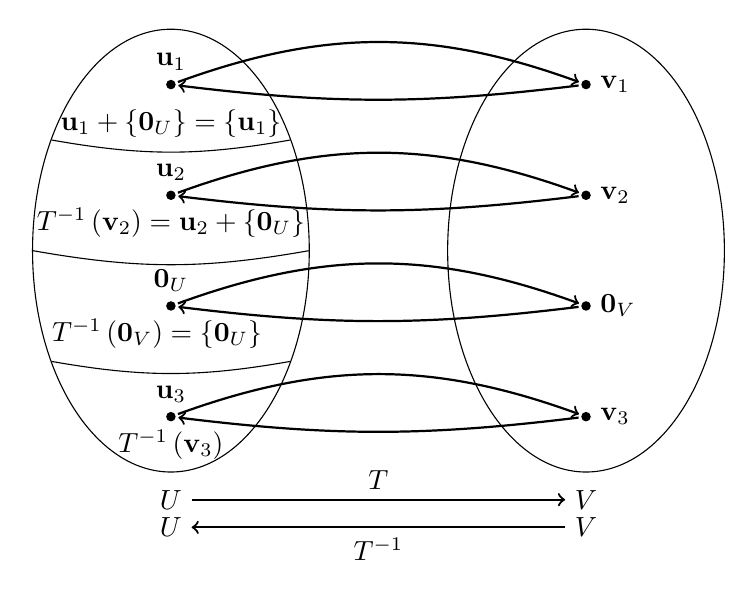
\begin{tikzpicture}
\tikzset{ltvect/.style={shape=circle, minimum size=0.30em, inner sep=0pt, draw, fill=black}}
\tikzset{ltedge/.style={->, bend left=20, thick, shorten <=0.1em, shorten >=0.1em}}
% base generic picture
\draw ( 5em, 8em) circle [x radius=5em, y radius=8em, thick];
\draw (20em, 8em) circle [x radius=5em, y radius=8em, thick];
\node (U) at ( 5em, -1em) {$U$};
\node (V) at (20em, -1em) {$V$};
\draw[->, thick, draw] (U) to node[auto] {$T$} (V);
% inputs
\node (u1)    [ltvect, label=above:$\vect{u}_1$]    at ( 5em, 14em) {};
\node (u2)    [ltvect, label=above:$\vect{u}_2$]    at ( 5em, 10em) {};
\node (zeroU) [ltvect, label=above:$\zerovector_U$] at ( 5em,  6em) {};
\node (u3)    [ltvect, label=above:$\vect{u}_3$]    at ( 5em,  2em) {};
% outputs
\node (v1)    [ltvect, label=right:$\vect{v}_1$]    at (20em, 14em) {};
\node (v2)    [ltvect, label=right:$\vect{v}_2$]    at (20em, 10em) {};
\node (zeroV) [ltvect, label=right:$\zerovector_V$] at (20em,  6em) {};
\node (v3)    [ltvect, label=right:$\vect{v}_3$]    at (20em,  2em) {};
% associations
\draw[ltedge] (u1) to (v1);
\draw[ltedge] (u2) to (v2);
\draw[ltedge] (zeroU) to (zeroV);
\draw[ltedge] (u3) to (v3);
% inverse associations
\draw[->, bend left=7, thick, shorten <=0.1em, shorten >=0.1em] (v1) to (u1);
\draw[->, bend left=7, thick, shorten <=0.1em, shorten >=0.1em] (v2) to (u2);
\draw[->, bend left=7, thick, shorten <=0.1em, shorten >=0.1em] (zeroV) to (zeroU);
\draw[->, bend left=7, thick, shorten <=0.1em, shorten >=0.1em] (v3) to (u3);
% preimages
\node (pre1) at (5em, 12.6em) {$\vect{u}_1 + \set{\zerovector_U}=\set{\vect{u}_1}$};
\node (pre2) at (5em,    9em) {$\preimage{T}{\vect{v}_2}=\vect{u}_2 + \set{\zerovector_U}$};
\node (pre3) at (4.5em,  5em) {$\preimage{T}{\zerovector_V}=\set{\zerovector_U}$};
\node (pre4) at (5em,    1em) {$\preimage{T}{\vect{v}_3}$};
% banding, x-coordinates are +/- 5*sqrt(3)/2 off midline
\node (b11) [minimum size=0em, inner sep=0pt] at (0.669873em, 12em) {};
\node (b12) [minimum size=0em, inner sep=0pt] at (9.330127em, 12em) {};
\node (b21) [minimum size=0em, inner sep=0pt] at (       0em,  8em) {};
\node (b22) [minimum size=0em, inner sep=0pt] at (      10em,  8em) {};
\node (b31) [minimum size=0em, inner sep=0pt] at (0.669873em,  4em) {};
\node (b32) [minimum size=0em, inner sep=0pt] at (9.330127em,  4em) {};
\draw [-, bend right=10] (b11) to (b12);
\draw [-, bend right=10] (b21) to (b22);
\draw [-, bend right=10] (b31) to (b32);
% inverse map
\node (UU) at ( 5em, -2em) {$U$};
\node (VV) at (20em, -2em) {$V$};
\draw[->, thick, draw] (VV) to node[auto] {$\ltinverse{T}$} (UU);
\end{tikzpicture}
\end{image}


Many will call an injective and surjective function a \dfn{bijective} function or just a \dfn{bijection}.  \ref{theorem:ILTIS} tells us that this is just a synonym for the term invertible (which we will use exclusively).



We can follow the constructive approach of the proof of \ref{theorem:ILTIS} to construct the inverse of a specific linear transformation, as the next example shows.



\begin{example}
[Computing the Inverse of a Linear Transformations]

Consider the linear transformation  $\ltdefn{T}{S_{22}}{P_2}$ defined by
\begin{align*}
\lteval{T}{\begin{bmatrix}a&b\\b&c\end{bmatrix}}
&=
\left(a+b+c\right)
+
\left(-a+2c\right)x
+
\left(2a+3b+6c\right)x^2
\end{align*}



$T$ is invertible, which you are able to verify, perhaps by determining that the kernel of $T$ is trivial and the range of $T$ is all of $P_2$.  This will be easier once we have \ref{theorem:RPNDD}, which appears later in this section.



By \ref{theorem:ILTIS} we know $\ltinverse{T}$ exists, and it will be critical shortly to realize that $\ltinverse{T}$ is automatically known to be a linear transformation as well (\ref{theorem:ILTLT}).  To determine the complete behavior of $\ltdefn{\ltinverse{T}}{P_2}{S_{22}}$ we can simply determine its action on a basis for the domain, $P_2$.  This is the substance of \ref{theorem:LTDB}, and an excellent example of its application.   Choose any basis of $P_2$, the simpler the better, such as $B=\set{1,\,x,\,x^2}$.  Values of $\ltinverse{T}$ for these three basis elements will be the single elements of their preimages.  In turn, we have
\begin{align*}
\preimage{T}{1}:&\\
&&\lteval{T}{\begin{bmatrix}a&b\\b&c\end{bmatrix}}
&=1+0x+0x^2\\
&&\begin{bmatrix}
 1 & 1 & 1 & 1\\
 -1 & 0 & 2 & 0\\
 2 & 3 & 6 & 0
\end{bmatrix}
&\rref
\begin{bmatrix}
1 & 0 & 0& -6 \\
0 & 1 & 0& 10 \\
0 & 0 & 1& -3
\end{bmatrix}
\\
&\text{(preimage)}&\preimage{T}{1}
&=\set{\begin{bmatrix}-6&10\\10&-3\end{bmatrix}}\\
&\text{(function)}&\lteval{\ltinverse{T}}{1}
&=
\begin{bmatrix}-6&10\\10&-3\end{bmatrix}\\
\preimage{T}{x}:&\\
&&\lteval{T}{\begin{bmatrix}a&b\\b&c\end{bmatrix}}
&=0+1x+0x^2\\
&&\begin{bmatrix}
 1 & 1 & 1 & 0\\
 -1 & 0 & 2 & 1\\
 2 & 3 & 6 & 0
\end{bmatrix}
&\rref
\begin{bmatrix}
1 & 0 & 0& -3 \\
0 & 1 & 0& 4 \\
0 & 0 & 1&  -1
\end{bmatrix}
\\
&\text{(preimage)}&\preimage{T}{x}
&=\set{\begin{bmatrix}-3&4\\4&-1\end{bmatrix}}\\
&\text{(function)}&\lteval{\ltinverse{T}}{x}
&=
\begin{bmatrix}-3&4\\4&-1\end{bmatrix}\\
\preimage{T}{x^2}:&\\
&&\lteval{T}{\begin{bmatrix}a&b\\b&c\end{bmatrix}}
&=0+0x+1x^2\\
&&\begin{bmatrix}
 1 & 1 & 1 & 0\\
 -1 & 0 & 2 & 0\\
 2 & 3 & 6 & 1
\end{bmatrix}
&\rref
\begin{bmatrix}
1 & 0 & 0& 2 \\
0 & 1 & 0& -3 \\
0 & 0 & 1&  1
\end{bmatrix}
\\
&\text{(preimage)}&\preimage{T}{x^2}
&=\set{\begin{bmatrix}2&-3\\-3&1\end{bmatrix}}\\
&\text{(function)}&\lteval{\ltinverse{T}}{x^2}
&=
\begin{bmatrix}2&-3\\-3&1\end{bmatrix}
\end{align*}




\ref{theorem:LTDB} says, informally, ``it is enough to know what a linear transformation does to a basis.''  Formally, we have the outputs of $\ltinverse{T}$ for a basis, so by \ref{theorem:LTDB} there is a unique linear transformation with these outputs.  So we put this information to work.  The key step here is that we can convert any element of $P_2$ into a linear combination of the elements of the basis $B$ (\ref{theorem:VRRB}).  We are after a ``formula'' for the value of $\ltinverse{T}$ on a generic element of $P_2$, say $p+qx+rx^2$.
\begin{align*}
\lteval{\ltinverse{T}}{p+qx+rx^2}
&=
\lteval{\ltinverse{T}}{p(1)+q(x)+r(x^2)}
&&\ref{theorem:VRRB}\\
&=
p\lteval{\ltinverse{T}}{1}+
q\lteval{\ltinverse{T}}{x}+
r\lteval{\ltinverse{T}}{x^2}
&&\ref{theorem:LTLC}\\
&=
p\begin{bmatrix}-6&10\\10&-3\end{bmatrix}+
q\begin{bmatrix}-3&4\\4&-1\end{bmatrix}+
r\begin{bmatrix}2&-3\\-3&1\end{bmatrix}\\
&=
\begin{bmatrix}
-6p-3q+2r & 10p+4q-3r \\
10p+4q-3r & -3p -q + r
\end{bmatrix}
\end{align*}




Notice how a linear combination in the domain of $\ltinverse{T}$ has been translated into a linear combination in the codomain of $\ltinverse{T}$ since we know $\ltinverse{T}$ is a linear transformation by \ref{theorem:ILTLT}.



Also, notice how the augmented matrices used to determine the three pre-images could be combined into one calculation of a matrix in extended echelon form, reminiscent of a procedure we know for computing the inverse of a matrix (see \ref{example:CMI}).  Hmmmm.



\end{example}

We will make frequent use of the characterization of invertible linear transformations provided by \ref{theorem:ILTIS}.  The next theorem is a good example of this, and we will use it often, too.



\begin{theorem}[Composition of Invertible Linear Transformations]
\label{theorem:CIVLT}


Suppose that $\ltdefn{T}{U}{V}$ and $\ltdefn{S}{V}{W}$ are invertible linear transformations.  Then the composition, $\ltdefn{\left(\compose{S}{T}\right)}{U}{W}$ is an invertible linear transformation.





\begin{proof}
Since $S$ and $T$ are both linear transformations,  $\compose{S}{T}$ is also a linear transformation by \ref{theorem:CLTLT}.    Since $S$ and $T$ are both invertible, \ref{theorem:ILTIS} says that $S$ and $T$ are both injective and surjective.  Then \ref{theorem:CILTI} says $\compose{S}{T}$ is injective, and \ref{theorem:CSLTS} says $\compose{S}{T}$ is surjective.  Now apply the ``other half'' of \ref{theorem:ILTIS} and conclude that $\compose{S}{T}$ is invertible.



\end{proof}
\end{theorem}

When a composition is invertible, the inverse is easy to construct.



\begin{theorem}[Inverse of a Composition of Linear Transformations]
\label{theorem:ICLT}


Suppose that $\ltdefn{T}{U}{V}$ and $\ltdefn{S}{V}{W}$ are invertible linear transformations. Then $\compose{S}{T}$ is invertible and

\begin{multipleChoice}
\choice[correct]{$\ltinverse{\left(\compose{S}{T}\right)}=\compose{\ltinverse{T}}{\ltinverse{S}}$.}
\choice{$\ltinverse{\left(\compose{S}{T}\right)}=\compose{\ltinverse{S}}{\ltinverse{T}}$.}
\end{multipleChoice}


\begin{proof}
Compute, for all $\vect{w}\in W$
\begin{align*}
\lteval{\left(\compose{\left(\compose{S}{T}\right)}{\left(\compose{\ltinverse{T}}{\ltinverse{S}}\right)}\right)}{\vect{w}}
&=\lteval{S}{\lteval{T}{\lteval{\ltinverse{T}}{\lteval{\ltinverse{S}}{\vect{w}}}}}\\
&=\lteval{S}{\lteval{I_V}{\lteval{\ltinverse{S}}{\vect{w}}}}&&\ref{definition:IVLT}\\
&=\lteval{S}{\lteval{\ltinverse{S}}{\vect{w}}}&&\ref{definition:IDLT}\\
&=\vect{w}&&\ref{definition:IVLT}\\
&=\lteval{I_W}{\vect{w}}&&\ref{definition:IDLT}
\end{align*}




So $\compose{\left(\compose{S}{T}\right)}{\left(\compose{\ltinverse{T}}{\ltinverse{S}}\right)}=I_W$, and also
\begin{align*}
\lteval{\left(\compose{\left(\compose{\ltinverse{T}}{\ltinverse{S}}\right)}{\left(\compose{S}{T}\right)}\right)}{\vect{u}}
&=\lteval{\ltinverse{T}}{\lteval{\ltinverse{S}}{\lteval{S}{\lteval{T}{\vect{u}}}}}\\
&=\lteval{\ltinverse{T}}{\lteval{I_V}{\lteval{T}{\vect{u}}}}&&\ref{definition:IVLT}\\
&=\lteval{\ltinverse{T}}{\lteval{T}{\vect{u}}}&&\ref{definition:IDLT}\\
&=\vect{u}&&\ref{definition:IVLT}\\
&=\lteval{I_U}{\vect{u}}&&\ref{definition:IDLT}
\end{align*}
so $\compose{\left(\compose{\ltinverse{T}}{\ltinverse{S}}\right)}{\left(\compose{S}{T}\right)}=I_U$.



By \ref{definition:IVLT}, $\compose{S}{T}$ is invertible and $\ltinverse{\left(\compose{S}{T}\right)}=\compose{\ltinverse{T}}{\ltinverse{S}}$.



\end{proof}
\end{theorem}

Notice that this theorem not only establishes \textit{what} the inverse of $\compose{S}{T}$ \textit{is}, it also duplicates the conclusion of \ref{theorem:CIVLT} and also establishes the invertibility of $\compose{S}{T}$.  But somehow, the proof of \ref{theorem:CIVLT} is a nicer way to get this property.


Does \ref{theorem:ICLT} remind you of the flavor of any theorem we have seen about matrices?  (Hint:  Think about getting dressed.)  Hmmmm.


\end{document}
